\documentclass[a4paper,11pt]{article}
\usepackage[a4paper, margin=8em]{geometry}

% usa i pacchetti per la scrittura in italiano
\usepackage[french,italian]{babel}
\usepackage[T1]{fontenc}
\usepackage[utf8]{inputenc}
\frenchspacing 

% usa i pacchetti per la formattazione matematica
\usepackage{amsmath, amssymb, amsthm, amsfonts}

% usa altri pacchetti
\usepackage{gensymb}
\usepackage{hyperref}
\usepackage{standalone}

\usepackage{colortbl}

\usepackage{xstring}
\usepackage{karnaugh-map}

% imposta il titolo
\title{Appunti Programmazione Avanzata}
\author{Luca Seggiani}
\date{2025}

% imposta lo stile
% usa helvetica
\usepackage[scaled]{helvet}
% usa palatino
\usepackage{palatino}
% usa un font monospazio guardabile
\usepackage{lmodern}

\renewcommand{\rmdefault}{ppl}
\renewcommand{\sfdefault}{phv}
\renewcommand{\ttdefault}{lmtt}

% circuiti
\usepackage{circuitikz}
\usetikzlibrary{babel}

% testo cerchiato
\newcommand*\circled[1]{\tikz[baseline=(char.base)]{
            \node[shape=circle,draw,inner sep=2pt] (char) {#1};}}

% disponi il titolo
\makeatletter
\renewcommand{\maketitle} {
	\begin{center} 
		\begin{minipage}[t]{.8\textwidth}
			\textsf{\huge\bfseries \@title} 
		\end{minipage}%
		\begin{minipage}[t]{.2\textwidth}
			\raggedleft \vspace{-1.65em}
			\textsf{\small \@author} \vfill
			\textsf{\small \@date}
		\end{minipage}
		\par
	\end{center}

	\thispagestyle{empty}
	\pagestyle{fancy}
}
\makeatother

% disponi teoremi
\usepackage{tcolorbox}
\newtcolorbox[auto counter, number within=section]{theorem}[2][]{%
	colback=blue!10, 
	colframe=blue!40!black, 
	sharp corners=northwest,
	fonttitle=\sffamily\bfseries, 
	title=Teorema~\thetcbcounter: #2, 
	#1
}

% disponi definizioni
\newtcolorbox[auto counter, number within=section]{definition}[2][]{%
	colback=red!10,
	colframe=red!40!black,
	sharp corners=northwest,
	fonttitle=\sffamily\bfseries,
	title=Definizione~\thetcbcounter: #2,
	#1
}

% disponi codice
\usepackage{listings}
\usepackage[table]{xcolor}

\definecolor{codegreen}{rgb}{0,0.6,0}
\definecolor{codegray}{rgb}{0.5,0.5,0.5}
\definecolor{codepurple}{rgb}{0.58,0,0.82}
\definecolor{backcolour}{rgb}{0.95,0.95,0.92}

\lstdefinestyle{codestyle}{
		backgroundcolor=\color{black!5}, 
		commentstyle=\color{codegreen},
		keywordstyle=\bfseries\color{magenta},
		numberstyle=\sffamily\tiny\color{black!60},
		stringstyle=\color{green!50!black},
		basicstyle=\ttfamily\footnotesize,
		breakatwhitespace=false,         
		breaklines=true,                 
		captionpos=b,                    
		keepspaces=true,                 
		numbers=left,                    
		numbersep=5pt,                  
		showspaces=false,                
		showstringspaces=false,
		showtabs=false,                  
		tabsize=2
}

\lstdefinestyle{shellstyle}{
		backgroundcolor=\color{black!5}, 
		basicstyle=\ttfamily\footnotesize\color{black}, 
		commentstyle=\color{black}, 
		keywordstyle=\color{black},
		numberstyle=\color{black!5},
		stringstyle=\color{black}, 
		showspaces=false,
		showstringspaces=false, 
		showtabs=false, 
		tabsize=2, 
		numbers=none, 
		breaklines=true
}


\lstdefinelanguage{assembler}{ 
  keywords={AAA, AAD, AAM, AAS, ADC, ADCB, ADCW, ADCL, ADD, ADDB, ADDW, ADDL, AND, ANDB, ANDW, ANDL,
        ARPL, BOUND, BSF, BSFL, BSFW, BSR, BSRL, BSRW, BSWAP, BT, BTC, BTCB, BTCW, BTCL, BTR, 
        BTRB, BTRW, BTRL, BTS, BTSB, BTSW, BTSL, CALL, CBW, CDQ, CLC, CLD, CLI, CLTS, CMC, CMP,
        CMPB, CMPW, CMPL, CMPS, CMPSB, CMPSD, CMPSW, CMPXCHG, CMPXCHGB, CMPXCHGW, CMPXCHGL,
        CMPXCHG8B, CPUID, CWDE, DAA, DAS, DEC, DECB, DECW, DECL, DIV, DIVB, DIVW, DIVL, ENTER,
        HLT, IDIV, IDIVB, IDIVW, IDIVL, IMUL, IMULB, IMULW, IMULL, IN, INB, INW, INL, INC, INCB,
        INCW, INCL, INS, INSB, INSD, INSW, INT, INT3, INTO, INVD, INVLPG, IRET, IRETD, JA, JAE,
        JB, JBE, JC, JCXZ, JE, JECXZ, JG, JGE, JL, JLE, JMP, JNA, JNAE, JNB, JNBE, JNC, JNE, JNG,
        JNGE, JNL, JNLE, JNO, JNP, JNS, JNZ, JO, JP, JPE, JPO, JS, JZ, LAHF, LAR, LCALL, LDS,
        LEA, LEAVE, LES, LFS, LGDT, LGS, LIDT, LMSW, LOCK, LODSB, LODSD, LODSW, LOOP, LOOPE,
        LOOPNE, LSL, LSS, LTR, MOV, MOVB, MOVW, MOVL, MOVSB, MOVSD, MOVSW, MOVSX, MOVSXB,
        MOVSXW, MOVSXL, MOVZX, MOVZXB, MOVZXW, MOVZXL, MUL, MULB, MULW, MULL, NEG, NEGB, NEGW,
        NEGL, NOP, NOT, NOTB, NOTW, NOTL, OR, ORB, ORW, ORL, OUT, OUTB, OUTW, OUTL, OUTSB, OUTSD,
        OUTSW, POP, POPL, POPW, POPB, POPA, POPAD, POPF, POPFD, PUSH, PUSHL, PUSHW, PUSHB, PUSHA, 
				PUSHAD, PUSHF, PUSHFD, RCL, RCLB, RCLW, MOVSL, MOVSB, MOVSW, STOSL, STOSB, STOSW, LODSB, LODSW,
				LODSL, INSB, INSW, INSL, OUTSB, OUTSL, OUTSW
        RCLL, RCR, RCRB, RCRW, RCRL, RDMSR, RDPMC, RDTSC, REP, REPE, REPNE, RET, ROL, ROLB, ROLW,
        ROLL, ROR, RORB, RORW, RORL, SAHF, SAL, SALB, SALW, SALL, SAR, SARB, SARW, SARL, SBB,
        SBBB, SBBW, SBBL, SCASB, SCASD, SCASW, SETA, SETAE, SETB, SETBE, SETC, SETE, SETG, SETGE,
        SETL, SETLE, SETNA, SETNAE, SETNB, SETNBE, SETNC, SETNE, SETNG, SETNGE, SETNL, SETNLE,
        SETNO, SETNP, SETNS, SETNZ, SETO, SETP, SETPE, SETPO, SETS, SETZ, SGDT, SHL, SHLB, SHLW,
        SHLL, SHLD, SHR, SHRB, SHRW, SHRL, SHRD, SIDT, SLDT, SMSW, STC, STD, STI, STOSB, STOSD,
        STOSW, STR, SUB, SUBB, SUBW, SUBL, TEST, TESTB, TESTW, TESTL, VERR, VERW, WAIT, WBINVD,
        XADD, XADDB, XADDW, XADDL, XCHG, XCHGB, XCHGW, XCHGL, XLAT, XLATB, XOR, XORB, XORW, XORL},
  keywordstyle=\color{blue}\bfseries,
  ndkeywordstyle=\color{darkgray}\bfseries,
  identifierstyle=\color{black},
  sensitive=false,
  comment=[l]{\#},
  morecomment=[s]{/*}{*/},
  commentstyle=\color{purple}\ttfamily,
  stringstyle=\color{red}\ttfamily,
  morestring=[b]',
  morestring=[b]"
}

\lstset{language=assembler, style=codestyle}

% disponi sezioni
\usepackage{titlesec}

\titleformat{\section}
	{\sffamily\Large\bfseries} 
	{\thesection}{1em}{} 
\titleformat{\subsection}
	{\sffamily\large\bfseries}   
	{\thesubsection}{1em}{} 
\titleformat{\subsubsection}
	{\sffamily\normalsize\bfseries} 
	{\thesubsubsection}{1em}{}

% tikz
\usepackage{tikz}

% float
\usepackage{float}

% grafici
\usepackage{pgfplots}
\pgfplotsset{width=10cm,compat=1.9}

% disponi alberi
\usepackage{forest}

\forestset{
	rectstyle/.style={
		for tree={rectangle,draw,font=\large\sffamily}
	},
	roundstyle/.style={
		for tree={circle,draw,font=\large}
	}
}

% disponi algoritmi
\usepackage{algorithm}
\usepackage{algorithmic}
\makeatletter
\renewcommand{\ALG@name}{Algoritmo}
\makeatother

% disponi numeri di pagina
\usepackage{fancyhdr}
\fancyhf{} 
\fancyfoot[L]{\sffamily{\thepage}}

\makeatletter
\fancyhead[L]{\raisebox{1ex}[0pt][0pt]{\sffamily{\@title \ \@date}}} 
\fancyhead[R]{\raisebox{1ex}[0pt][0pt]{\sffamily{\@author}}}
\makeatother

\begin{document}
% sezione (data)
\section{Lezione del 23-09-25}

% stili pagina
\thispagestyle{empty}
\pagestyle{fancy}

% testo
\subsection{Introduzione}
Il corso di programmazione avanzata si pone di approfondire gli aspetti di programmazione \textit{orientata agli oggetti} (\textbf{OOP}) e \textit{concorrente}, sfruttando sia come strumento che come fine il linguaggio di programmazione \textbf{Java}.
Parleremo sia di programmazione desktop che applicazioni in rete (cioè servizi per pagine Web).

\subsubsection{Cenni storici}
Java nasce nei primi anni '90 come \textit{Oak} all'interno della \textit{Sun Microsystems} (poi acquisita da Oracle).

L'idea originale del progetto era quella di realizzare un linguaggio per la programmazione di dispositivi di elettronica di consumo.
Per questo motivo una delle prime prerogative del progetto era che il linguaggio potesse creare programmi che giravano su una variegata gamma di piattaforme hardware (il cosiddetto paradigma \textbf{WORA}, \textit{Write Once, Run Anywhere}).

Con l'avvento del Web e delle applicazioni distribuite in modello client-server, l'obiettivo del progetto virò verso la creazione di un linguaggio che potesse essere eseguito sui client, all'interno dei browser (nei cosiddetti \textit{applet}), a scapito dell'architettura o il S/O locale (browser Netscape su architetture non-Intel e S/O Unix come browser Explorer su architetture Intel e S/O Microsoft).

Oggi questo tipo di uso è in declino, ma il linguaggio Java rimane estremamente popolare per lo sviluppo di applicazioni desktop/mobile, e in contesto sopratutto aziendale per lo sviluppo di applicazioni lato server.

\subsubsection{Versioni}
Possiamo individuare alcune versioni di rilevo dello standard Java.
\begin{itemize}
	\item Nel 1996 viene lanciata la JDK 1.0 (\textit{Java Development Kit}), prima versione del linguaggio;
	\item Nel 1998 viene lanciata la J2SE 1.2, da cui la denominazione \textit{Java 2}, rimasta fino alla 5.0 del 2004 (fra l'altro slegata in nome dalla versione precedente, la 1.4);
	\item Dal 2006 vengono usate le denominazioni Java SE 6 e successive, ed è stato adottato un modello di rilascio periodico (da Java SE 9 annuale).
		Questo è più o meno in corrispondenza dell'acquisto da parte di Oracle di Sun Microsystems, avvenuto nel 2010 (la prima versione lanciata sotto la Oracle fu Java SE 7).
\end{itemize}

Nel progetto originale della Sun Microsystems erano previste più \textit{edizioni} di Java, fra cui:
\begin{itemize}
	\item Java \textbf{ME}, cioè \textit{Micro Edition}, che mirava a piattaforme con risorse limitate;
	\item Java \textbf{SE}, cioè \textit{Standard Edition}, che mirava a piattaforme desktop;
	\item Java \textbf{EE}, cioè \textit{Enterprise Edition}, che mirava a piattaforme distribuite e in rete.
\end{itemize}

Java è fornito sia come \textbf{JDK} (come già detto \textit{Java Development Kit}), comprensivo di compilatore e strumenti di sviluppo, che come \textbf{JRE} (\textit{Java Runtime Environment}), pensato solo per l'esecuzione di applicazioni già sviluppate.

Notiamo poi che noi useremo la piattaforma \textbf{OpenJDK}, implementazione open source del JDK lanciata da Sun Microsystems nel 2006, prima dell'acquisizione da parte di Oracle, e ancora oggi mantenuta da Oracle ma comunque mantenuta open source. 

\subsubsection{Natura del Java}
I design goal di Java sono i seguenti: 
\begin{itemize}
	\item Semplice, paradigma orientato agli oggetti e familiare per gli sviluppatori di linguaggi precedenti (si pensi alla famiglia C/C++, con cui condivide sintassi e diversi costrutti);
	\item Robusto e sicuro, in particolare riguardo alla memoria (non sono presenti meccanismi come i puntatori, e la gestione della memoria è quindi \textit{sicura} e largamente fuori dalle mani del programmatore);
	\item \textit{Architecture-neutral}, cioè neutrale all'architettura e portatile su una vasta gamma di piattaforme (come già detto, paradigma \textit{WORA}). In questo, la specifica non contiene ambiguità (i tipi, ad esempio, sono standardizzati in dimensioni, a differenza del C++ che è \textit{platform-dependent}).

		Il codice sorgente Java viene compilato nel cosiddetto \textbf{bytecode}, una sorta di codice macchina che viene eseguito sulla \textbf{JVM}, una macchina virtuale basata sullo \textit{stack} piuttosto che su \textit{registri}, e agnostica al livello fisico sottostante;
	\item Alte prestazioni, difficili da ottenere a causa della sua natura sostanzialmente interpretata, ma comunque quasi paragonabili nelle ultime versioni a codice scritto con linguaggi come C/C++, sopratutto nel caso di codice che viene ripetuto molte volte.
		Questo è reso possibile anche dall'uso di tecnologie di compilazione \textbf{JIT} (compilazione \textit{Just In Time}).

		Come nota storica, vediamo che sono state sviluppate implementazioni hardware della JVM, oggi non più particolarmente in voga;
	\item Interpretato, \textit{threaded}, cioè ottimizzato per l'esecuzione su sistemi \textit{multithreaded}, e dinamico per quanto riguarda il collegamento delle librerie, che viene effettuato a tempo di esecuzione.
\end{itemize}

Abbiamo quindi che le differenza principali fra i linguaggi C/C++ a cui siamo abituati e il Java sono:
\begin{itemize}
	\item La natura dinamica del Java (anche le classi possono essere caricate a tempo di esecuzione);
	\item Il supporto nativo per il multithreading, che in Java è praticamente immediato, mentre in C++ richiede API e tecniche di programmazione considerevolmente più complesse.
\end{itemize}

\subsubsection{Java e Android}
Un caso di applicazione di Java degno di nota è quello dello sviluppo di applicazioni per il sistema operativo Android.

Android era infatti fornito nelle prime versioni della macchina virtuale \textbf{Dalvik}, basata sui registri, che esegue codice Java compilato in un bytecode apposito, appunto il codice \textit{Dalvik} (da cui \lstinline|.dex|, \textit{Dalvin EXecutable}).

Il supporto per la macchina Dalvik è rimasto in Android fino alla versione 4.4 \textit{KitKat}, ed è stato seguito nella 5.0 \textit{Lollipop} da \textbf{ART} (\textit{Android RunTime}), che usa lo stesso bytecode e gli stessi eseguibili, ma con diverse ottimizzazioni.

Notiamo poi che oggi (dal 2019) Android è una piattaforma \textit{Kotlin-first}, cioè orientata al linguaggio "successore" del Java, il \textbf{Kotlin}.

\subsection{Ciao mondo in Java}
Possiamo quindi vedere il nostro primo programma di esempio in Java.
\begin{lstlisting}[language=java, style=codestyle]	
class Main {
	public static void main(String[] args) {
		System.out.println("C# is better");
	}
}
\end{lstlisting}

Vediamo come tutto sta necessariamente dentro una classe, qui la classe \lstinline|Main|, che definisce un metodo, qui il metodo \lstinline|main()|.

Questo metodo è specifico (come il \lstinline|main()| del C/C++), viene eseguito quando la classe che lo possiede è invocata come programma, e ha come argomento la lista degli argomenti programma \lstinline|String[] args|, dove le quadre definiscono un'array come per la normale sintassi c-like.
Inoltre, il metodo \lstinline|main()| è dichiarato come:
\begin{itemize}
	\item \lstinline|public|, cioè chiunque può invocarlo;
	\item \lstinline|static|, cioè appartiene alla definizione di classe stessa, e non ad una particolare istanza di classe.
\end{itemize}

Da qui usiamo la funzione di libreria \lstinline|println| per stampare un messaggio a video.

Possiamo compilare questo codice inserendolo in un file col nome della classe definita, \lstinline|Main.java|, e compilare come:
\begin{lstlisting}[style=shellstyle]
javac Main.json
\end{lstlisting}
Questo creerà un nuovo file, \lstinline|Main.class|, contenente appunto la classe \lstinline|Main|.
A questo punto si esegue come:
\begin{lstlisting}[style=shellstyle]
java Main
\end{lstlisting}
notando che si riporta solo il nome della classe, senza l'estensione \lstinline|.java|.

\subsection{Tipi del Java}
Il Java è un linguaggio fortemente tipizzato dove ogni oggetto ha un tipo.
In particolare notiamo fra tipi \textbf{primitivi} e di \textbf{riferimento}.

\newpage

\begin{itemize}
	\item I tipi \textbf{primitivi} sono i classici tipi di dato disponibili negli altri linguaggi:
\begin{lstlisting}[language=java, style=codestyle]	
int x;
float y = 5.6;
double pippo = 3.2 + Math.sqrt(7.4);
int i1, i2, i3;
char a = 'a';
// String s = "Also try Kotlin";
/* const int VAL; no ! */ 
static final int VAL; // e' effettivamente costante
\end{lstlisting}
La lista completa dei tipi è la seguente:
	\begin{table}[H]
		\center \rowcolors{2}{white}{black!10}
		\begin{tabular} { c | c }
			\bfseries Tipo & \bfseries Descrizione \\
			\hline
			\lstinline|boolean| & Un booleano \lstinline|true| o \lstinline|false| \\ 
			\lstinline|char| & Un carattere, cioè un \textit{codepoint} UTF-16 su 16 bit \\ 
			\lstinline|byte| & Un intero su 8 bit \\ 
			\lstinline|short| & Un intero su 16 bit \\ 
			\lstinline|int| & Un intero su 32 bit \\ 
			\lstinline|long| & Un intero su 64 bit \\ 
			\lstinline|float| & Un numero in virgola mobile su 32 bit come definito da IEEE 754 \\ 
			\lstinline|double| & Un numero in virgola mobile su 64 bit come definito da IEEE 754 \\ 
		\end{tabular}
	\end{table}
		Notiamo innanzitutto che il Java adotta la codifica UTF-8 per le stringhe e UTF-16 per i caratteri. Ricordiamo poi che, come già detto, i tipi del Java (ad esempio i tipi numerici) hanno dimensione fissata dalla specifica e non \textit{platform-specific}.

	Vediamo poi che la parola chiave \lstinline|const| non è implementata in Java (anche se è comunque riservata), mentre sono disponibili le parole chiave \lstinline|static| e \lstinline|final|. In particolare questa assegna a variabili valori finali, cioè che non possono più essere alterati.

	I valori non inizializzati in Java vengono lasciati in uno stato \lstinline|undefined|, possono restare tali fino alla definizione, ma se si prova ad usarli prima il compilatore lancia un errore.

	Per ogni tipo primitivo esiste poi un corrispondente \textit{tipo oggetto}, cioè sostanzialmente una classe \textit{wrapper} per quel tipo di primitivo. 

	\par\medskip
	\textbf{\textsf{Conversioni fra tipi}} \\
	\noindent
	La conversione fra tipi primitivi e oggetto corrispondenti è automatica.
	Sono poi previste le conversioni implicite fra tipi primitivi secondo i meccanismi che ci aspettiamo:

	\begin{center}	
		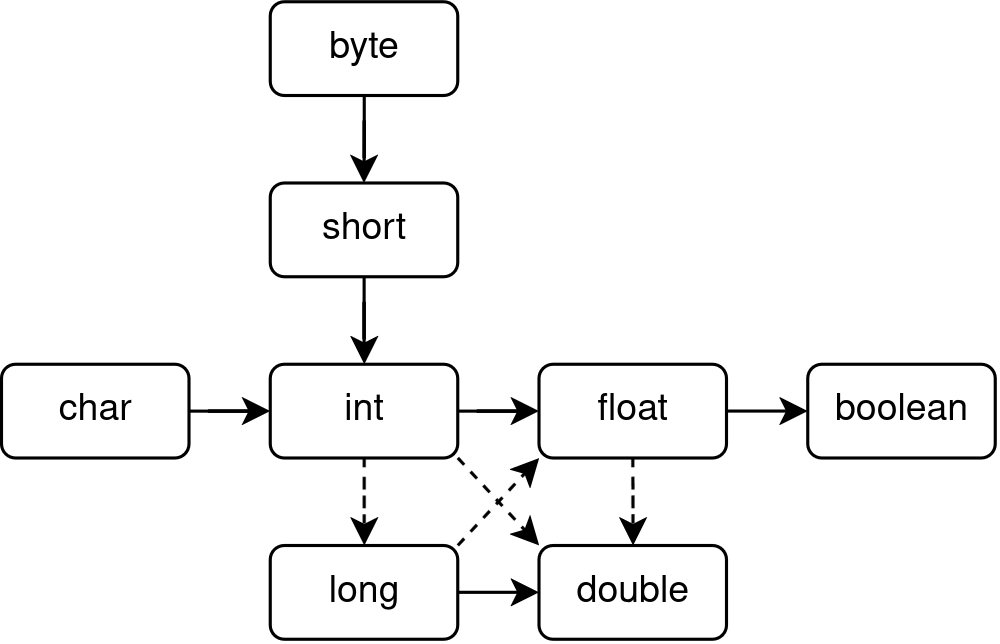
\includegraphics[scale=0.3]{../figures/conversioni_implicite.png}
	\end{center}

	Per effettuare cast nelle direzioni opposte a quelle previste dalle conversioni implicite si usano le conversioni esplicite secondo la solita sintassi:
\begin{lstlisting}[language=java, style=codestyle]	
float pi = 3.14;
int engineer_pi = (int) pi; // engineer_pi = 3
\end{lstlisting}

	\item I tipi di \textbf{riferimento} comprendono:
		\begin{itemize}
			\item Array;
			\item Classi;
			\item Interfacce.
		\end{itemize}
\end{itemize}

\subsubsection{Costrutti del Java}
Il Java comprende tutti i costrutti condizionali e di ripetizione a cui siamo abituati.
Notiamo in particolare la presenza del costrutto \textit{for-each} disponibile come:
\begin{lstlisting}[language=java, style=codestyle]	
for(tipo variabile : espressione_insieme) {
	// corpo
}
\end{lstlisting}
che itera sugli elementi dell'oggetto \lstinline|set_expression| instanziandoli ogni volta nell'oggetto \lstinline|variabile|.

Vediamo quindi tutti i costrutti disponibili:

\noindent
\begin{minipage}[t]{0.45\textwidth}
\begin{table}[H]
	\center 
	\begin{tabular} { c | p{.1cm} p{5cm} }
		\bfseries Costrutto & \bfseries Sintassi \\ 
		\hline 
\lstinline|if-else| & & \begin{lstlisting}[language=java, style=codestyle]	
if(espressione) {
	// vera
} else {
	// falsa
}
\end{lstlisting} \\
\lstinline|switch| & & \begin{lstlisting}[language=java, style=codestyle]	
switch(espressione) {
	case a: // caso a
	case b: // caso b
	// ...
	default: // caso default
}
\end{lstlisting} \\
\lstinline|while| & & \begin{lstlisting}[language=java, style=codestyle]	
while(espressione) {
	// corpo
}
\end{lstlisting} \\
\lstinline|do-while| & & \begin{lstlisting}[language=java, style=codestyle]	
do {
	// corpo
} while(espressione);
\end{lstlisting} \\
	\end{tabular}
\end{table}
\end{minipage}%
\hfill
\begin{minipage}[t]{0.45\textwidth}
\begin{table}[H]
	\center 
	\begin{tabular} { c | p{.1cm} p{5cm} }
		\bfseries Costrutto & \bfseries Sintassi \\ 
		\hline 
\lstinline|for| & & \begin{lstlisting}[language=java, style=codestyle]	
for(espressione; espressione; espressione) {
	// corpo
}
\end{lstlisting} \\
\lstinline|for-each| & & \begin{lstlisting}[language=java, style=codestyle]	
for(tipo variabile : espressione_insieme) {
	// corpo
}
\end{lstlisting} \\
\lstinline|break| & & \begin{lstlisting}[language=java, style=codestyle]	
break;
\end{lstlisting} \\
\lstinline|continue| & & \begin{lstlisting}[language=java, style=codestyle]	
continue;
\end{lstlisting} \\
	\end{tabular}
\end{table}
\end{minipage}

\subsubsection{Classe \lstinline|System|}
\lstinline|System| è una classe delle librerie Java dotata di 3 campi per la gestione degli stream di I/O:
\begin{itemize}
	\item \lstinline|System.in|, che gestisce il flusso di ingresso (tastiera).
		Per l'ingresso inglobiamo lo stream \lstinline|System.in| all'interno della classe \lstinline|Scanner| come segue:
\begin{lstlisting}[language=java, style=codestyle]	
Scanner s = new Scanner(System.in);
\end{lstlisting}
A questo punto possiamo usare i metodi della classe scanner come \lstinline|next()| (che si ferma alla parola) e \lstinline|nextLine()| (che si ferma alla riga) per leggere dallo stream.
Vediamo che la classe \lstinline|Scanner| è la prima che incontriamo a non essere inclusa di default nel sorgente, ma che va inclusa con la direttiva \lstinline|import|:
\begin{lstlisting}[language=java, style=codestyle]	
import java.util.Scanner;

// classe main, ecc... 
\end{lstlisting}
	\item \lstinline|System.out|, che gestisce il flusso di uscita (video). Sono disponibili i metodi \lstinline|println()|, e \lstinline|print()| (che non stampa i caratteli di ritorno carrello e nuova linea);
	\item \lstinline|System.err|, che gestisce il flusso di errore (sempre video);
\end{itemize}

\subsection{Classi del Java}
In Java \textit{tutto} il codice è dentro classi.
Una classe contiene:
\begin{itemize}
	\item La definizione della struttura degli oggetti (istanze) della classe attraverso le \textit{variabili istanza};
	\item La definizione della struttura dei dati comuni ad ogni classe attraverso le \textit{variabili classe}.
\end{itemize}
Queste strutture vengono definite con:
\begin{itemize}
	\item Variabili possedute dalla classe (\textbf{campi});
	\item Codice che manipola gli oggetti, o in particolare i membri di classe (\textbf{metodi} e non \textit{funzioni});
	\item I meccanismi per la costruzione di oggetti (\textbf{costruttori}).
\end{itemize}
Variabili e funzioni di classe (cioè campi e metodi) sono anche detti \textbf{membri}.

Una classe in Java si istanzia sempre con la parola chiave \lstinline|new|, in quanto non si possono allocare classi Java sullo stack, solo sull'heap.
Abbiamo quindi che:
\begin{lstlisting}[language=java, style=codestyle]	
Classe cl1;
\end{lstlisting}
non istanzia alcuna classe, ma esiste solo come un oggetto \textit{riferimento} a oggetti di tipo \lstinline|Classe|, che colleghiamo ad un oggetto vero e proprio sull'heap come:
\begin{lstlisting}[language=java, style=codestyle]	
Classe cl1 = new Classe(/* argomenti del costruttore */);
\end{lstlisting}

Il fatto che gli oggetti dichiarati come \lstinline|Classe| sono solo riferimenti ad oggetti sull'heap significa che facendo cose come \lstinline|cl1 = cl2| stiamo solo spostando il riferimento da un oggetto all'altro, e non copiando le variabili istanza dei singoli oggetti.

Per accedere alle variabili istanza usiamo la classica notazione a punto (\lstinline|Classe.variabile|, ecc...).
Nessuno ci nega di includere riferimenti ad altre classi come membri di classi, dobbiamo solo ricordare che stiamo parlando sempre di riferimenti e non di oggetti classe veri e propri.

\subsubsection{Costruttori}
I costruttori sono sequenze di istruzioni utilizzate per definire lo stato iniziale di un oggetto in fase di instanziazione (quando viene usata la \lstinline|new|), nel caso questo sia necessario, cioè i meccanismi standard non sono sufficienti (costruttore di default nullo) o ci sono informazioni note solo al momento della \lstinline|new|.

I costruttori del Java:
\begin{itemize}
	\item Hanno lo stesso nome della classe;
	\item Non restituiscono valore;
	\item Possono essere eseguiti solo in occasione della \lstinline|new|;
	\item Possono avere 0 o più argomenti.
\end{itemize}

\end{document}
